\documentclass[12pt,a4paper,twoside]{book}

% Remove footnote line
\renewcommand{\footnoterule}{}
\usepackage{pre}

%%% TITLE PAGE %%%

\title
    {
    \vspace{-2.5cm}
        {
\includegraphics[width=.215\textwidth]{figs/PWrLogo.eps}} \par \vspace{1ex} \large{WROCŁAW UNIVERSITY OF SCIENCE AND TECHNOLOGY} 
	\par \vspace{1ex}
	{\scshape\large Faculty of Fundamental Problems of Technology\par}
	\vspace{2cm}
    {Bachelor thesis\par}  % Preserve either Bachelor or Master, not both.
    \vspace{2cm}
	{\Large{\bf Clinical decision support system for renal dose adjustment based on Summary of Product Characteristics}}
    }
    
\author
    {
    \vspace{1cm}
    Author: Tsimur Halkin\\
    Supervisor: dr hab. inż. Sebastian Kraszewski
    }
\date{\vfill Wrocław~2026}

%%% BEGINNING OF THE THESIS %%%

\begin{document}

\maketitle

\afterpage{\blankpage}\clearpage

\begin{flushright}
    \thispagestyle{empty}
    \vspace*{\fill}
    
    {\em To my \dots}  % parents etc.
    % \vspace*{\fill}
\end{flushright}

\afterpage{\blankpage}\clearpage

{
  \hypersetup{linkcolor=black}
  \tableofcontents
}

%%%%%%%%%%%%%%%%%%%%%%%%%%%%%%%%%%%%%%
% IT IS GOOD TO WRITE EACH SENTENCE IN A SEPARATE LINE,
% BECAUSE THIS HELPS FIND A PARTICULAR SENTENCE BY SIMPLY
% EYE-SCANNING THE LEFT EDGE OF THE .TEX FILE.
% IT IS ALSO EASY TO SWITCH ON/OFF A PARTICULAR SENTENCE BY COMMENTING IT OUT.
% BESIDES, IN REAL-TIME DISCUSSIONS ONE CAN REFER TO 
% A PARTICULAR SENTENCE BY A SPECIFIC LINE OF THE .TEX FILE.
%%%%%%%%%%%%%%%%%%%%%%%%%%%%%%%%%%%%%%

\chapter{Introduction}\label{ch:intro}

\section{Project Background and Motivation}\label{sec:background-motivation}

Renal impairment can significantly change how drugs are handled by the body. 
For some medicines, reduced kidney function may require a lower dose, a longer dosing interval, additional monitoring, or even avoiding the drug. 
In everyday clinical work, this information is usually checked manually in Summary of Product Characteristics .

These documents are official and reliable, but they are not convenient for automatic use. 
They are usually available as PDF files, and relevant information may be spread across different sections, such as dosage, contraindications, warnings, and pharmacokinetics. 
This makes renal dose checking repetitive and time-consuming, especially when a patient receives several drugs at the same time.

This project was motivated by the idea that official drug information can be organized into a structured knowledge base and used by a software system to support renal dose adjustment. 
The goal is not to replace clinical judgement, but to make the lookup process more transparent, consistent, and easier to review.

\section{Goal of the Thesis}\label{sec:goal-thesis}

This thesis presents the design and implementation of a prototype clinical decision support system for renal dose adjustment. 
The system uses structured rules derived from Summary of Product Characteristics documents and applies them to basic patient data and a medication list.

The main goal is to generate explainable recommendations based on validated rules. 
For each drug, the system should indicate whether standard dosing can be used, whether dose adjustment or monitoring is needed, whether the drug should be avoided, or whether manual review is required. 
Each recommendation should also point to the source document and section from which the rule was derived.

The final recommendation is produced by a deterministic rule-based engine. 
AI may be used as a \textbf{helper} for extracting candidate rules from ChPL documents, but it does not directly decide the final recommendation.


\section{Problem Statement}\label{sec:problem-statement}

Information about renal dose adjustment is available in official Summary of Product Characteristics%
\footnote{In Poland, the Summary of Product Characteristics is known as \textit{Charakterystyka Produktu Leczniczego} (ChPL). It is an official document describing the approved conditions of use of a medicinal product, including dosage, contraindications, warnings, and pharmacological properties.}, 
but it is not provided in a structured form suitable for automatic decision support.

For each drug, the relevant information may appear in different sections of the document, including dosage, contraindications, warnings, and pharmacokinetic properties. 
Moreover, recommendations may depend on the route of administration, pharmaceutical form, renal function threshold, or the presence of severe renal impairment.

The central problem addressed in this thesis is the transformation of textual drug information from ChPL documents into structured, validated decision rules that can be used by a software system. 
The system must be able to calculate renal function, match the calculated value with appropriate rules, and present the result in an explainable way. 
If a reliable rule is not available, the system should avoid guessing and indicate that manual clinical review is required.

Therefore, the project combines three technical challenges: extraction and organization of information from official product documents, representation of renal dosing knowledge in a database, and deterministic rule-based generation of recommendations.

\section{Project Assumptions}\label{sec:project-assumptions}

The project is based on several assumptions that define the intended use and technical boundaries of the prototype. 
First, Summary of Product Characteristics documents are treated as the primary source of drug dosing information. 
Only information derived from these documents is used to create renal dosing rules stored in the system knowledge base.

Second, the final recommendation is generated by a deterministic rule-based engine. 
The system does not allow an AI model to directly decide the dose or override validated rules. 
AI may be used only as a helper for processing ChPL documents and suggesting candidate rules, which must be reviewed before they become active in the system.

Third, the prototype uses a limited set of selected drugs instead of attempting to cover all medicines available in clinical practice. 
The selected drugs are used to demonstrate the complete workflow: document analysis, rule creation, renal function calculation, rule matching, and recommendation generation.

Fourth, the system works with synthetic patient data only. 
The prototype is not connected to hospital systems, electronic health records, or real clinical databases. 
Patient parameters are entered manually in order to test the decision workflow in a controlled environment.

Fifth, the system assumes that renal dose adjustment can be represented as structured rules based on renal function thresholds, recommendation types, and source references. 
If no validated rule is available for a given drug, route, or renal function range, the system should not guess the recommendation and should instead indicate that manual review is required.

Finally, the prototype is designed as an academic and engineering demonstration. 
It is not intended for real clinical use, does not replace the judgement of a physician or pharmacist, and is not certified as medical device software.

%%%%%%%%%%%%%%%%%%%%%%%%%%%%%%%%%%%%

\chapter{Background}
\section{Renal Dose Adjustment}
\label{sec:renal-dose-adjustment}

Renal dose adjustment is the modification of drug therapy according to the patient's kidney function. 
It is necessary because impaired renal function can reduce the elimination of drugs or active metabolites and increase the risk of toxicity. 
Depending on the medicine, renal impairment may require a lower dose, a longer dosing interval, additional monitoring, avoidance of the drug, or manual clinical review. 
The need for adjustment depends not only on the degree of renal impairment, but also on drug-specific factors, such as the fraction eliminated by the kidneys, the presence of active metabolites, the therapeutic index, and the risk of adverse effects~\cite{artDooguePolasek2011DrugDosingRenalDisease,artStefani2019AdjustDrugDosesCKD}.

\paragraph{Glomerular filtration and its estimation.}
Each nephron begins with a glomerulus, a network of capillaries through which water and small dissolved substances pass from blood plasma into the renal tubule.
Blood cells and most proteins remain in the circulation.
The tubule subsequently returns much of the filtered water and useful solutes to the blood and secretes additional substances into the tubular fluid.
Together, these processes allow the kidneys to remove waste while regulating the body's water and electrolyte balance~\cite{miscNIDDKKidneys}.

The glomerular filtration rate (GFR) is the volume of filtrate formed by all functioning glomeruli per unit time.
In routine practice, a blood sample can be used to estimate this rate from the serum concentration of creatinine, a waste product of muscle metabolism.
With stable creatinine production and kidney function, a lower filtration rate generally corresponds to a higher serum creatinine concentration.
Muscle mass and tubular secretion also influence that concentration, so two people with the same serum creatinine can have different filtration rates~\cite{miscNIDDKDrugDosing}.
The term \emph{estimated GFR} (eGFR) refers to the result of an estimating equation.

\paragraph{The two estimates used in RenalSafe.}
The 2021 creatinine equation from the Chronic Kidney Disease Epidemiology Collaboration (CKD-EPI) estimates GFR from age, sex, and standardized serum creatinine~\cite{artInker2021CKDEPI}.
Let \(A\) be age in years, \(\mathrm{SCr}\) the numerical value of serum creatinine in \(\mathrm{mg/dL}\), and \(x=\mathrm{SCr}/\kappa\).
Then
\begin{equation}
    \mathrm{eGFR}_{\mathrm{cr}} =
    142\,\min(x,1)^{\alpha}\,\max(x,1)^{-1.200}\,0.9938^{A}\,f ,
    \label{eq:implemented-ckd-epi}
\end{equation}
where the female coefficients are \(\kappa=0.7\), \(\alpha=-0.241\), and \(f=1.012\), and the male coefficients are \(\kappa=0.9\), \(\alpha=-0.302\), and \(f=1\).
The result is expressed in \(\mathrm{mL/min}\) per \(1.73\,\mathrm{m}^{2}\) of body surface area.
Indexing to this reference surface area allows filtration estimates to be compared across individuals of different sizes~\cite{miscNIDDKDrugDosing}.

Some prescribing information specifies thresholds in terms of estimated creatinine clearance (CrCl)~\cite{artDowling2010RenalDrugDosing,artJones2011RenalFunctionDrugDosing}.
Creatinine clearance is the volume of plasma from which the kidneys clear creatinine per unit time.
Because the tubules secrete some creatinine in addition to the amount filtered at the glomerulus, creatinine clearance can exceed GFR~\cite{artJones2011RenalFunctionDrugDosing}.
The Cockcroft--Gault equation estimates CrCl in \(\mathrm{mL/min}\) as
\begin{equation}
    \mathrm{CrCl} = \frac{(140-A)\,W}{72\,\mathrm{SCr}}\,c ,
    \label{eq:cockcroft-gault}
\end{equation}
where \(W\) is body weight in kilograms and \(c\) is \(0.85\) for females and \(1\) for males~\cite{artCockcroftGault1976}.
Both equations use serum creatinine in \(\mathrm{mg/dL}\). A concentration reported in \(\mu\mathrm{mol/L}\) is converted by dividing its numerical value by \(88.4\).

\paragraph{Relevance to dosing.}
When filtration declines, a drug that depends substantially on glomerular filtration for elimination may accumulate if the same dose is repeated at the same interval~\cite{artDooguePolasek2011DrugDosingRenalDisease}.
The product information links a renal function range to a dosing instruction, so the choice of estimate matters particularly near a threshold~\cite{artStevens2009DrugDosingRecommendations,artHudsonNolin2018KidneyFunctionDrugDosing}.
For example, when a rule specifies Cockcroft--Gault CrCl in \(\mathrm{mL/min}\), comparing its threshold directly with an indexed CKD-EPI value would change both the quantity and the units being compared.
RenalSafe therefore records the required metric with each rule and requests manual review when that estimate is unavailable.

\section{Summary of Product Characteristics as a Data Source}
\label{sec:smpc-data-source}

The Summary of Product Characteristics (SmPC), known in Poland as \textit{Charakterystyka Produktu Leczniczego} (ChPL), is an official document describing the approved conditions of use of a medicinal product. 
According to the European Medicines Agency, the SmPC is the basis of information for healthcare professionals on how to use a medicine safely and effectively~\cite{miscEMASmPC}. 
For this reason, ChPL documents are a natural source of knowledge for a system that supports drug dosing decisions.

The structure of an SmPC is standardized. 
For renal dose adjustment, the most relevant parts are usually section 4.2, which describes posology and method of administration, section 4.3, which lists contraindications, section 4.4, which contains special warnings and precautions, and section 5.2, which describes pharmacokinetic properties. 
The European Commission guideline on SmPC presentation describes the expected structure and principles for presenting information in these documents~\cite{miscEuropeanCommissionSmPCGuideline}. 
In practice, renal impairment may be mentioned in more than one section, for example as a precise dose adjustment table in section 4.2, as a warning in section 4.4, or as information about renal elimination in section 5.2.

In Poland, information about authorised medicinal products is available through the official Rejestr Produktów Leczniczych. 
The register contains information about medicinal products authorised for use in Poland, and its public data files may include links to product leaflets and ChPL documents~\cite{miscURPLRPL,miscEZdrowieRPLXML}. 
This makes it possible to treat ChPL documents not only as individual PDF files, but also as a potential source for a structured drug knowledge base.

However, ChPL documents are not designed primarily for automatic decision support. 
They are usually distributed as PDF or text documents intended for human reading. 
Relevant dosing information may be written as free text, placed in tables, repeated across sections, or expressed using different renal function metrics such as creatinine clearance or eGFR. 
Recommendations may also depend on the pharmaceutical form, route of administration, dose strength, age group, or clinical context. 
Therefore, the same active substance cannot always be represented by a single universal rule.

For the prototype developed in this thesis, ChPL documents are treated as the primary source of renal dosing rules, but not as directly executable logic. 
The information extracted from them must first be transformed into a structured representation containing the drug product, route of administration, renal function metric, renal function range, recommendation type, source section, and validation status. 
Only validated rules are used by the recommendation engine. 
This approach keeps the final decision process traceable to official product information while still allowing the system to operate on structured data.

\section{Clinical Decision Support Systems}\label{sec:cdss}

A clinical decision support system (CDSS) is a type of healthcare software that combines patient-specific information with medical knowledge in order to support clinical decision-making~\cite{artBates2003TenCommandments}. 
In contrast to general healthcare data platforms, a CDSS is not mainly focused on storing or moving data, but on interpreting it in a specific clinical context and returning an output that can be used by the clinician.

In this thesis, the supported clinical decision is limited to renal dose adjustment. 
The system receives basic patient parameters and a medication list, calculates renal function, and compares the result with validated dosing rules derived from Summary of Product Characteristics documents. 
The output belongs to one of several recommendation categories: \textit{standard dose}, \textit{adjust dose or interval}, \textit{additional monitoring}, \textit{avoid}, or \textit{manual review required}.

Renal dosing is a suitable use case for decision support, because several studies have shown that inappropriate dosing is common in patients with reduced kidney function~\cite{artDowling2010RenalDrugDosing,artStevens2009DrugDosingRecommendations}. 
Computerized dosing support was also shown to improve the appropriateness of prescriptions for patients with renal insufficiency in selected clinical settings~\cite{artChertow2001GuidedMedicationDosing,artTerrell2010CDSSRenalDosing}. 
These findings give a practical motivation for building a prototype that applies renal dosing rules in a structured and traceable way.

CDSS implementations can be described using several practical distinctions. 
A system may be \textit{active} or \textit{passive}, depending on whether it automatically generates alerts or responds only to an explicit user request. 
It may also be \textit{embedded} into an electronic health record workflow or operate as a \textit{standalone} tool. 
Finally, it may be \textit{knowledge-driven}, using validated rules, or \textit{data-driven}, using models trained on historical data.

The prototype developed in this thesis is intentionally designed as a passive, standalone, knowledge-driven system. 
It is passive because the physician explicitly enters patient data and asks for a recommendation. 
It is standalone because it is not integrated with hospital information systems or electronic health records. 
It is knowledge-driven because recommendations are generated by a deterministic rule-based engine using validated rules stored in the knowledge base, not by a model trained on historical clinical data.

Explainability is an important requirement for this type of system. 
A recommendation should show which rule was applied, which patient value matched the rule, and which source document supports the recommendation. 
This requirement directly influences the data model: every renal dosing rule stored in the knowledge base contains a reference to the source document and to the section from which it was derived.

Another important design issue is the risk of non-actionable or excessive alerts. 
Drug safety alerts are frequently overridden in clinical practice, and high override rates have been reported in computerized physician order entry systems~\cite{artVanderSijs2006Override}. 
For this reason, the prototype follows a conservative answering policy. 
If no validated rule matches the drug, route of administration, and renal function range, the system does not try to infer a recommendation and instead returns \textit{manual review required}. 
This behaviour is consistent with the principle that decision support should be actionable, transparent, and fitted to the user's workflow~\cite{artBates2003TenCommandments}.
\section{Healthcare Data Platforms and Polish E-Health Context}
\label{sec:healthcare-data-platforms}

Modern clinical decision support systems are usually not isolated applications. 
In real healthcare environments, decision support depends on access to structured data, reliable source documents, integration mechanisms, audit logs, and controlled user access. 
For this reason, many enterprise systems follow a platform-oriented approach, where data from multiple sources is accumulated, normalized, analysed, governed, and then used to support operational decisions.

Examples of such platform-oriented systems include Palantir Foundry and Snowflake. 
Palantir Foundry provides tools for data integration and uses an ontology layer to organize data, models, and operational objects into a shared representation of an organization~\cite{miscPalantirFoundryDataIntegration,miscPalantirFoundryOntology}. 
Snowflake represents a cloud data platform approach that supports data storage, analytics, engineering workflows, applications, and data sharing within a managed environment~\cite{miscSnowflakeAIDataCloud}. 
Although these systems are not clinical decision support systems by themselves, they illustrate an important architectural pattern: data ingestion, structured storage, governance, analytics, and user-facing workflows can be combined within one platform.

This type of architecture is relevant to healthcare because clinical data is often distributed across many systems and must be transformed before it can be used for decision-making. 
A similar platform-oriented direction can also be observed in modern healthcare interoperability standards. 
For example, the HL7 FHIR Clinical Reasoning module describes how clinical knowledge artifacts, such as decision support rules, protocols, and quality measures, can be represented and exchanged between healthcare systems~\cite{miscHL7FHIRClinicalReasoning}. 
This shows that decision support is not only a matter of implementing algorithms, but also of organizing knowledge, data, and workflow integration.

A comparable digital transformation can be observed in the Polish healthcare system. 
The national e-health system, known as P1, provides digital services such as electronic prescriptions, electronic referrals, electronic medical documentation, medical events, e-registration, the Internet Patient Account, the mojeIKP application, and gabinet.gov.pl~\cite{miscEZdrowieP1}. 
These services support patients, medical professionals, healthcare providers, and public administration, showing that healthcare in Poland is increasingly based on structured digital data exchange.

The prototype developed in this thesis is not integrated with national e-health infrastructure and does not process real patient data. 
However, its internal architecture follows a simplified version of the same general idea. 
Drug information is imported from official source documents, transformed into structured rules, stored in a knowledge base, and then used by a decision engine to generate explainable recommendations. 
In this sense, the system can be treated as a small domain-specific decision support platform focused only on renal dose adjustment.


\section{Rule-Based and AI-Assisted Decision Support}
\label{sec:rule-ai-decision-support}

Decision support systems can use different approaches to generate recommendations. 
In this thesis, the final recommendation is produced by a rule-based decision engine. 
This means that the system does not learn dosing decisions from historical patient data, but applies explicitly defined rules stored in the knowledge base. 
For the renal dosing problem, such rules connect a drug product, route of administration, renal function metric, renal function range, and recommendation type.

A rule-based approach is suitable for this prototype for several reasons. 
First, renal dosing recommendations from ChPL documents are often expressed as thresholds or categories, for example for patients with creatinine clearance below a given value. 
Second, rule-based decisions are easier to test and explain than black-box model outputs. 
Third, every recommendation can be traced back to a specific source document and section. 
This is important in a medical-informatics system, where the user should be able to understand why a recommendation was returned and which source supports it.

A dosing rule states when a recommendation applies.
For example, a rule for a fictional intravenous medicine might read, \emph{If creatinine clearance is at least 30 but below 50~mL/min, give doses farther apart.}
For that product, route, form, and indication, a clearance of 40~mL/min falls within the range, while 50~mL/min falls outside it.
When exactly one approved rule applies, RenalSafe displays its recommendation and the passage in the product information that supports it.
If the system cannot identify a single applicable rule, it displays \emph{manual review required}.

Artificial intelligence can still be useful in this project, but its role is different. 
ChPL documents are usually written as human-readable text and may contain tables, section references, and non-uniform wording. 
Because of this, extracting renal dosing information from them may be time-consuming. 
An AI-assisted module may help identify relevant fragments of text, suggest candidate renal thresholds, classify recommendation types, or produce a structured draft rule. 
Recent work on large language models for drug-label and drug-safety information extraction shows that such models can support extraction tasks from regulatory drug documents, but also that their outputs require careful validation~\cite{artWu2025AskFDALabel,artGisladottir2025DrugSafetyLLM}.

In the proposed architecture, AI-generated outputs are therefore treated only as candidate rules. 
They are stored with a pending validation status and cannot be used by the recommendation engine until they are reviewed and approved. 
This separation is important because large language models may misinterpret source text, omit conditions, confuse units, or overinterpret ambiguous information. 
Reviews of large language models in medicine emphasize that, although these systems may be useful in clinical and biomedical workflows, reliability, hallucination risk, and human oversight remain important concerns~\cite{artJung2025LLMsMedicine,artAsgari2025LLMHallucinationSafety}.

The final decision workflow is therefore hybrid but conservative. 
AI may support document processing, while the actual recommendation is generated only from validated structured rules. 
This design keeps the most safety-critical part of the system deterministic, explainable, and auditable. 
It also fits the engineering scope of the thesis: the objective is not to train a new clinical model, but to build a prototype that transforms official drug information into a structured knowledge base and applies it through a transparent decision process.
%%%%%%%%%%%%%%%%%%%%%%%%%%%%%%%%%%%%%%

\chapter{Requirements and Dataset}
\section{Functional Requirements}
\section{Non-Functional Requirements}
\section{Selected Drug Groups}
\section{Source Documents and Manual Rule Preparation}

%%%%%%%%%%%%%%%%%%%%%%%%%%%%%%%%%%%%%%%%%%%%%%%%%%%%%%%%

\chapter{System Design}
\section{General System Architecture}
\label{sec:general-system-architecture}

RenalSafe is implemented as a standalone web application with three main components: a browser-based user interface, an application backend, and a relational database.
The interface is developed in React and TypeScript, while the backend is written in Go.
The Go service exposes a REST API and serves the compiled interface, so the browser communicates with a single application service.
PostgreSQL with the pgvector extension stores source documents, structured rules, synthetic patient records, assessment results, and audit events.

Figure~\ref{fig:renalsafe-architecture} shows how the Go service connects the browser to the database and where the optional extraction provider enters the workflow.

\begin{figure}[htbp]
    \centering
    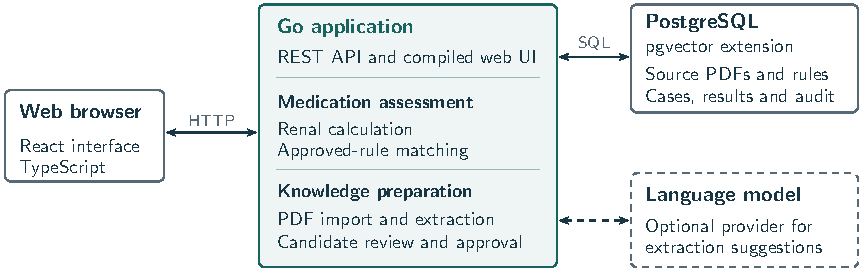
\includegraphics[width=\linewidth]{figs/renalsafe-architecture.pdf}
    \caption[RenalSafe system architecture]{RenalSafe system architecture. The Go application and PostgreSQL run in separate containers. The dashed connection carries extraction requests and suggestions for review. Medication assessments use the approved rules stored in PostgreSQL.}
    \label{fig:renalsafe-architecture}
\end{figure}

The backend separates renal function calculation, rule matching, document processing, and persistence into distinct modules within one application.
The renal calculator derives estimates from the supplied patient parameters.
The decision engine evaluates approved rules against the medication context and the renal function metric required by each rule.
A successful match returns the rule's recommendation and source reference; missing information or the absence of a unique applicable rule results in a manual-review status.
The engine does not call a language model, and its explanations are constructed from the calculation, matched rule, and supporting source evidence.

Knowledge preparation follows a separate workflow within the same service.
PDF text is extracted using Poppler, and candidate rules can be prepared manually or suggested by an optional language-model provider.
Model-assisted extraction is handled by a background worker in the Go application.
Suggestions must be explicitly saved as pending candidates and reviewed by a pharmacist before they can be approved for use by the decision engine.
This separation allows assessments based on existing approved rules to operate without the model provider.

The local deployment consists of an application container and a database container managed by Docker Compose.
The implemented architecture supports demonstration with synthetic patient data; clinical validation and model-quality evaluation are separate from the implementation described here.

\section{Decision Models}
\label{sec:decision-models}

RenalSafe evaluates each medication in an assessment against the renal function metric specified by its approved rules.
The calculator computes the available estimates once for the patient. These can include Cockcroft--Gault creatinine clearance in \(\mathrm{mL/min}\) and the 2021 CKD-EPI creatinine estimate of glomerular filtration rate in \(\mathrm{mL/min}/1.73\,\mathrm{m}^{2}\).
Their availability depends on the inputs. For example, if the other inputs pass validation but body weight is missing, the calculator can still return an indexed eGFR. A medication whose rules require creatinine clearance then receives a manual-review result.

The engine first selects approved rules that exactly match the product, route of administration, pharmaceutical form, and indication.
These rules must specify a single renal metric. The engine compares the unrounded estimate for that metric with each rule's interval, respecting whether each endpoint is included.
Exactly one interval must contain the estimate. The rule's approval must also be effective at the assessment time, and the patient must satisfy any age or weight conditions recorded in the rule.
If any of these checks fails, the result identifies the reason for manual review and contains no dosing action.

The distinction between a point estimate and a range matters near a threshold. In a synthetic software test, two creatinine clearance rules cover \([0,30)\) and \([30,\infty)\) in \(\mathrm{mL/min}\). A value of exactly \(30\) matches the second rule.
If the request also supplies lower and upper bounds for serum creatinine, the calculator propagates both through the equation. When the resulting clearance interval extends across the threshold, the engine returns manual review even though the point estimate alone matches one rule.

A successful match returns the action recorded in the rule (no change, reduce dose, extend interval, avoid use, or use with caution), together with its source citation and any dosing instructions stored in the rule.
Checking a proposed prescription is a separate, optional decision. For an avoidance rule, the engine flags the proposed use as outside the rule limits. For other actions, it can compare the entered single dose and dosing interval with an explicit maximum single dose and minimum interval.
If those limits are absent or the dose units differ, the prescription check requires manual review. The user can therefore see which adjustment rule applies even when the system cannot assess the proposed regimen.

\section{Knowledge Base Design}
\label{sec:knowledge-base-design}

Figure~\ref{fig:knowledge-base-schema} shows how a dosing rule can be traced to the text that supports it.
Its passage reference identifies the section and page containing the quotation, while its document reference identifies the edition of the SmPC.
For example, if a dosing table lists three renal intervals in the same passage, each interval can have its own rule while all three rules refer to the same passage and document.

\begin{figure}[htbp]
    \centering
    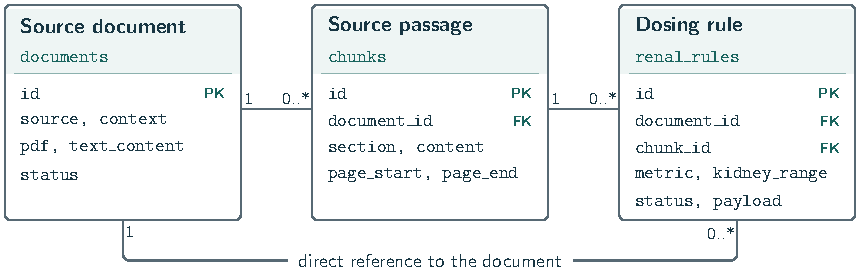
\includegraphics[width=\linewidth]{figs/knowledge-base-schema.pdf}
    \caption[Knowledge base schema]{Core knowledge base tables and selected columns. Each passage belongs to one document, and each rule cites one passage and one document. The label \texttt{0..*} means zero or more related records. PK denotes a primary key and FK a foreign key.}
    \label{fig:knowledge-base-schema}
\end{figure}

The \texttt{documents} table stores the original PDF and its extracted text alongside the medication context, source URL, version, retrieval time, and a SHA-256 digest for each representation.
The \texttt{chunks} table records the section, physical page range, byte offsets in the extracted text, and passage content. Full-text search and optional vector search operate on these passages.
When a reviewer saves a candidate rule, the quoted text must occur exactly once in the selected passage. The application uses the position of that occurrence to determine the physical page, so a reviewer can locate the same wording in the stored PDF.

The \texttt{renal\_rules} table links each rule to its document and passage. It stores the medication context, metric, renal interval, and review status in columns, and preserves the complete rule, including the action, optional conditions, and citation, in a JSON payload.
A database constraint prevents two approved rules for the same medication context and metric from covering a common value. It permits gaps, which the decision engine handles through manual review as described in Section~\ref{sec:decision-models}.

New candidates enter review as pending. A pharmacist approves or rejects a specific candidate by submitting its content digest and a review note. Approval also requires explicit confirmation and records the reviewer's identity and the time of approval.
This ties the decision to the version the pharmacist inspected. If another user edits the pending candidate before the review is submitted, the digest changes and the earlier review cannot be applied.
When a source document is superseded by another for the same medication context, the application marks its pending and approved rules as superseded in the same database transaction. Subsequent assessments use the active sources, while earlier assessments retain the rule and citation originally returned.

\section{Recommendation Workflow}
\label{sec:recommendation-workflow}

In the patient workspace, the physician opens an active synthetic case and selects the creatinine observation to use for the assessment.
If the measurement has yet to be recorded, the physician enters its value, unit, and sample time, together with its standardization status and any known uncertainty bounds.
The assessment form displays these laboratory fields as read-only.
On submission, the server reads them from the selected observation and verifies that it still belongs to the case and has not been superseded by a correction.

The physician enters the patient's age and the sex used by the renal equations, supplies weight and height when available, and confirms the clinical conditions relevant to the calculation.
For each medication, the physician selects a catalogue entry specifying the product, pharmaceutical form, route, and indication.
Selecting a medication is sufficient to request its applicable adjustment rule.
To check a proposed regimen as well, the physician enters both the single dose with its unit and the interval between doses.

When the physician selects \emph{Calculate and save assessment}, the server evaluates the medications against a single knowledge-base snapshot using the decision model described in Section~\ref{sec:decision-models}.
The result page shows the renal estimates and a separate outcome for each medication.
For a match, the physician can inspect the action, any dosing instructions, and the supporting SmPC passage.
For manual review, the page gives the reason, such as an unavailable renal metric.
Consequently, one medication can have a documented recommendation while another in the same assessment still requires review.

The server saves the inputs, results, knowledge snapshot, link to the observation, and audit events in one transaction.
If the same submission is retried with its original request key, the physician receives the existing assessment.
The case history also supports recalculation after a laboratory correction.
For example, if a transcription error is discovered, the physician records a replacement observation and can use it in a new assessment linked to the earlier one.
Both results remain available for comparison, each with the measurement and rules used at the time.

\section{AI-Assisted Rule Extraction Workflow}


%%%%%%%%%%%%%%%%%%%%%%%%%%%%%%%%%%%%%%%%%%%%%%%%%%%%%%%%
\chapter{Implementation}
\section{Technology Stack}
\label{sec:technology-stack}

Docker Compose runs the RenalSafe application and its PostgreSQL database as two local services.
Building the application requires a larger set of tools than running it.
Table~\ref{tab:technology-stack} identifies the role of each technology in the implementation.

\begin{table}[htbp]
    \centering
    \caption[RenalSafe technology stack]{Technologies used to build and run RenalSafe, as specified in the application repository at revision \texttt{9c3cc33}.}
    \label{tab:technology-stack}
    \begin{tabularx}{\linewidth}{@{}l >{\raggedright\arraybackslash}X@{}}
        \toprule
        \textbf{Technology} & \textbf{Role in RenalSafe} \\
        \midrule
        React 19 and TypeScript 5.9 & Implement the browser interface for patient cases, medication assessments, and rule review. \\
        Node.js 22 and Vite 8 & Run the frontend build and bundle the browser assets. \\
        Go 1.25 & Implements the HTTP API, renal calculations, rule evaluation, and database access through the \texttt{pgx} driver. \\
        PostgreSQL 18 & Stores documents, rules, and assessment history. The \texttt{pgvector} extension supports passage search by embedding similarity. \\
        Poppler & Provides \texttt{pdftotext} for extracting UTF-8 text from imported SmPC files while retaining their page layout as far as possible. \\
        Docker Compose & Starts the application and database containers and attaches a persistent volume to PostgreSQL. \\
        \bottomrule
    \end{tabularx}
\end{table}

The browser and the Go service share an OpenAPI description of the requests and responses exchanged through the API.
For example, the assessment form uses TypeScript types generated from this description when it submits a medication list and reads the saved result.
During the container build, the frontend build script regenerates the type definitions, checks them against the copy in the repository, and type-checks the interface before Vite bundles it.
The Go build then embeds the resulting assets in the server executable.
This lets the browser load the interface and submit assessments to the same origin, with Node.js needed only at build time.

The storage layer uses different PostgreSQL features for passage retrieval and rule matching.
Evidence retrieval can rank passages using full-text search or stored embeddings.
Rule matching uses explicit renal intervals, represented in PostgreSQL by the \texttt{numrange} type.
A database exclusion constraint uses \texttt{btree\_gist} to combine equality on medication context and metric with an overlap check on the interval, enforcing the approval condition described in Section~\ref{sec:knowledge-base-design}.

\section{Backend Implementation}
\label{sec:backend-implementation}

The Go backend separates HTTP request handling, database operations, and assessment logic into the \texttt{httpapi}, \texttt{store}, and \texttt{decision} packages.
The patient assessment described in Section~\ref{sec:recommendation-workflow} illustrates how the three packages interact.
A physician submits the identifier of a stored creatinine observation together with the current patient parameters and medication list.
The HTTP handler checks the caller's role and decodes the JSON body into a typed request.
The decoder rejects unknown fields and repeated keys, so a request containing two different creatinine values under the same key is rejected before it reaches the calculator.

The handler passes the authenticated caller, patient identifier, and request to \texttt{AssessPatient} in the store package.
For a new assessment, this method checks access to the case and retrieves the selected observation only if it belongs to the patient and has not been superseded.
It copies the creatinine value, unit, sample time, standardization status, and any uncertainty bounds from that record into the assessment input.
The store then loads a versioned knowledge snapshot and passes it with the completed request to \texttt{decision.Assess}.
The decision function operates on these two inputs in memory, which also allows the same function to run in unit tests without an HTTP server or database.

One PostgreSQL transaction saves the assessment, its knowledge snapshot, the link to the observation, and the corresponding audit events.
The handler returns HTTP~201 with the saved record's location after the transaction commits.
This distinction matters if the browser loses the response after a successful save.
On a retry, the store looks up the request key for the same physician and patient and compares a digest of the submitted data with the stored digest.
An identical submission returns the existing record. Reusing the key with changed inputs produces HTTP~409, leaving the original assessment available in the case history.

\section{Renal Function Calculator}
\label{sec:renal-function-calculator}

The \texttt{renal.Calculate} function accepts the patient parameters and an explicit assessment time.
It normalizes the measurement and any supplied bounds to \(\mathrm{mg/dL}\) using the conversion in Section~\ref{sec:renal-dose-adjustment}.
It then checks the inputs against the prototype's adult, stable-renal-function policy.
The policy accepts ages from 18 through 120 years and a sample taken no more than seven days before the assessment.
It requires a supported equation sex, a standardized creatinine measurement, confirmation of stable renal function and typical body composition, and explicit exclusion of suspected acute kidney injury and dialysis.
A missing confirmation or a sample dated after the assessment yields a warning and an empty set of estimates.
The age and time limits describe the operating scope chosen for this prototype.

After the shared input checks pass, the calculator evaluates Equation~\eqref{eq:implemented-ckd-epi} and records the result as indexed eGFR.
It additionally evaluates Equation~\eqref{eq:cockcroft-gault} when actual body weight is confirmed and height is available for the body size check.
Height is required by the implementation for its body mass index check, although height does not appear in the equation itself.
When both weight and height are supplied, a body mass index outside the prototype interval of \(18.5\) to \(30\,\mathrm{kg/m^2}\) blocks both estimates.
If height alone is missing and the other supplied inputs pass validation, the calculator returns indexed eGFR with a warning that creatinine clearance is unavailable.

Each returned estimate carries its metric identifier, unit, formula version, point value, and bounds.
When the request includes a creatinine interval, both endpoints must be included and the interval must contain the reported measurement.
For fixed patient parameters, both equations decrease as creatinine rises, so the upper creatinine bound gives the lower renal estimate and the lower creatinine bound gives the upper estimate.
For example, in the synthetic calculator fixture for a 70-year-old male weighing \(72\,\mathrm{kg}\), a creatinine concentration of \(1.0\,\mathrm{mg/dL}\) gives a Cockcroft--Gault estimate of \(70\,\mathrm{mL/min}\).
With input bounds of \(0.9\) and \(1.1\,\mathrm{mg/dL}\), the corresponding clearance bounds are approximately \(63.6\) and \(77.8\,\mathrm{mL/min}\).
The calculator passes the unrounded values to the decision engine for the interval check described in Section~\ref{sec:decision-models}.

\section{Rule-Based Recommendation Engine}
\label{sec:recommendation-engine}

The Go function \texttt{decision.Assess} implements the matching procedure described in Section~\ref{sec:decision-models}.
It accepts a request and a validated knowledge snapshot, calls the renal calculator once, and constructs one result for each medication in request order.
Each result starts with the status \texttt{MANUAL\_REVIEW\_REQUIRED}.
If a check fails, the function appends the reason to that result and continues with the next medication.
For instance, when the required estimate is unavailable, the result includes the calculator's warnings as well as the reason that matching stopped.
This lets the caller distinguish a missing weight measurement from a gap in the approved rules.

For each medication, the function scans the snapshot for approved rules whose product, route, form, and indication match the request exactly.
It collects the distinct renal metrics used by those rules before comparing any values.
Even if the calculator produced both estimates, the engine requests review when the eligible rules specify different metrics.
Once it has identified a single metric, it uses the interval method \texttt{Contains} to compare its unrounded point estimate against each rule's lower and upper bounds, including or excluding each endpoint as specified.
After finding a unique point match, the engine checks the approval date, any age or weight conditions, and whether the same interval contains both bounds returned by the calculator.

Only after these checks succeed does the function set \texttt{RULE\_MATCHED} and copy the action and any dosing instructions from the rule.
It builds the explanation from the selected estimate, rule identifier and version, and the cited SmPC section, page, and quotation.
When the request includes a proposed prescription, its medication index identifies the result to which the separate prescription check belongs.
For a rule with explicit regimen limits, the comparison tests whether the single dose exceeds the stored maximum or the interval falls below the stored minimum.
Equality at either limit is allowed. A difference in dose units requires manual review, even when the rule itself matched.
The saved assessment includes the engine and calculator policy versions, together with the knowledge version and digest, so the inputs to a later replay can be identified.

\section{Document Processing Module}
\label{sec:document-processing}

The document processing module turns an uploaded SmPC into passages that a reviewer can trace back to the original PDF.
The upload contains the PDF and metadata identifying the medication context, source URL, document version, and first and last physical pages for that product.
The page range matters when one PDF contains information for several products because a heading such as SmPC section~4.2 can occur more than once.

The Go service passes the PDF bytes to Poppler's \texttt{pdftotext} utility, requesting UTF-8 text with the page layout retained.
The extractor accepts PDFs up to 12~MiB, limits extracted output to 16~MiB, and sets a 30-second timeout.
If a scan produces too little text, the import fails and requires manual preparation or optical character recognition before it can proceed.
For a successful extraction, the parser uses the page-break characters in the text to locate the declared page range.
Within that range, it looks for numbered headings 4.1--4.9, 5.1, and 5.2.
Each section records its physical page range and its starting and ending byte offsets in the full extracted text.

Long sections are split at paragraph boundaries with a target of 6000~bytes per passage.
Dosing tables need special care because a row can depend on a unit in the heading or a qualification in a footnote.
The splitter uses aligned whitespace to identify possible table blocks and groups them with adjacent paragraphs before choosing a split point.
An indivisible block can therefore exceed the target length.
This heuristic preserves surrounding text for inspection. Interpreting a column or verifying what a footnote qualifies remains a review task.

During import, the store computes separate SHA-256 digests for the PDF and extracted text and writes the document, passages, knowledge revision update, and audit event in one transaction.
The byte offsets allow a passage to be checked by taking the corresponding slice of the stored UTF-8 text, including Polish characters that occupy more than one byte.
When a reviewer later saves a candidate rule, the quotation must occur exactly once in the selected passage.
Counting page breaks before that occurrence gives the physical page on which the quotation starts, completing the link from the rule to the PDF shown in Figure~\ref{fig:knowledge-base-schema}.

\section{User Interface}


%%%%%%%%%%%%%%%%%%%%%%%%%%%%%%%%%%%%%%%%%%%%%%%%%%%%%%%%

\chapter{Testing and Evaluation}
\section{Testing Strategy}
\section{Synthetic Patient Cases}
\section{Evaluation of Rule Matching}
\section{Example Recommendations}

%%%%%%%%%%%%%%%%%%%%%%%%%%%%%%%%%%%%%%%%%%%%%%%%%%%%%%%%
\chapter{Conclusions}
\section{Summary of Results}
\section{Limitations}

The prototype is limited to a selected set of drugs and manually validated rules.
It does not cover all medicines available in clinical practice and does not attempt
to replace full pharmaceutical review.
The system uses synthetic patient cases and is not integrated with hospital
information systems or electronic health records. Therefore, the evaluation is
technical and functional rather than clinical.
The system relies on information extracted from ChPL documents. Although
these documents are official sources, their structure is not always convenient for
automatic processing, especially when information is provided as free text or
tables.
AI-assisted extraction, if used, is treated only as a support mechanism. Can-
didate rules requires clinical validation before they can be used by the recommendation engine.
\section{Future Work}

%%%%%%%%%%%%%%%%%%%%%%%%%%%%%%%%%%%%%%
\chapter{Discussion}\label{ch:disco}

A well written thesis should contain a well written discussion of the results obtained, with references to the exiting literature as well as to the aim of the thesis.

%%%%%%%%%%%%%%%%%%%%%%%%%%%%%%%%%%%%%%

\bibliographystyle{plain}
\bibliography{refs}

\appendix

\renewcommand*\listfigurename{List of figures} 
\hypersetup{linkcolor=black}
\listoffigures

\renewcommand*\listtablename{List of tables} 
\hypersetup{linkcolor=black}
\listoftables

\end{document}